%This is the fourth chapter of the dissertation

%The following command starts your chapter. If you want different titles used in your ToC and at the top of the page throughout the chapter, you can specify those values here. Since Columbia doesn't want extra information in the headers and footers, the "Top of Page Title" value won't actually appear.

\pagestyle{cu}
\graphicspath{{./Chapter4/Figures/}}
\chapter[Purity and the Electron Lifetime][Purity and the Electron Lifetime]{Purity and the Electron Lifetime}

In a noble element dark matter detection experiment the purity of the target mass is an essential consideration and must be measured
continuously.  To date the concentration of electronegative impurities has always been measured in these experiments, but no reliable
model has existed to explain and predict its behavior.

In this chapter I discuss the necessity of extremely pure xenon (\secref{}), explain the original model fit to XENON1T data
(\secref{}), and examine how abrupt changes in detector conditions alter the contamination (\secref{}).



\section{Importance and Procedure for Purifying Xenon}
\secref{sec:importance_procedure}
Purity usually refers to two distinct but correlated values, though the degree of the correlation can depend on the
experiment.  The first is radioactive elements of other noble elements that cannot be completely removed during distillation.  For xenon
our primary challenges are \ce{^{85}Kr} (\secref{subsubsec:backgrounds_electronic_krypton}) and \ce{^{222}Rn}
(\secref{subsubsec:backgrounds_electronic_radon}) as they have low-energy decays that can contaminate our region of interest (while
\ce{^{220}Rn} also leads to a low-energy \betadecay its half-life is too short to penetrate our detector and thus can be ignored).

The second consideration with regards to detector purity is contamination of electronegative impurities such as \ce{O_2} or
\ce{N_2}.  These attach to drifting electrons, lowering or even eliminating the S2.  This can have the largest impact at low energies
since the number of \electron is much fewer.  To correct for the expected initial number of electrons we can use the electron lifetime
$\tau_{\mathrm{e^-}}$, though this must be monitored consistently if not perpetually.  Of course, if the entire cloud of electrons is
removed by these impurities we cannot apply a correction since we have no knowledge of where in the detector it occurred or the energy
deposition.

This chapter is focused on the latter of these two purities, though its examination necessitates consideration of the former as we will
see.



\subsection{Effects of Electronegative Impurities}
\label{subsec:importance_procedure_effects}
Electronegative impurities decrease the photons and electrons measured.

\subsubsection{Photon Attenuation}
\label{subsubsec:importance_procedure_effects_photons}
Contaminants been shown to absorb Xe scintillation (178 nm with ${\sim} 14\ \mathrm{nm}$ spectral FWHM)
(\citeref{Watanabe1953a, Watanabe1953b}).  At concentrations of ppm or higher
the fraction of UV photons that reach the PMTs can be considerably decreased - especially for large detectors.  The intensity due to
photon attenuation is given by

\begin{equation}
I(x) = I_0 e^{-x / \lambda_{\mathrm{att}}}
\end{equation}

\nonindent where $I_0$ is initial intensity, $x$ is distance, and $\lambda_{\mathrm{att}}$ is the attenuation length.  It can be written
as $1 / \lambda_{\mathrm{att}} = 1 / \lambda_{\mathrm{abs}} + 1 / \lambda_{\mathrm{scatt}}$ where $\lambda_{\mathrm{abs}}$ and
$\lambda_{\mathrm{scatt}}$ are the the absorption and scatterings lengths, respectively.  For entirely pure xenon
$\lambda_{\mathrm{abs}} \sim \infty$ (\citeref{Baldini2005} found $lambda_{\mathrm{abs}} > 100\ \mathrm{cm}$ at 90\% confidence
level).

The inclusion of impurities, however, can shorten the absorption
length.  \figerf{fig:importance_procedure_effects_photons_absorption_coefficents} shows the absorption coefficients
($\lambda_{\mathrm{abs}}^{-1}$) for 1 ppm \htwoo and \otwo from $130 \mdash 200\ \mathrm{nm}$.  They overlap with shorter wavelengths
of the xenon spectrum (included for comparison), meaning measured VUV photons by PMTs will not be symmetric above 178 nm.  With a nearly
1-meter tall detector a 1 ppm concentration of \htwoo would have an effect at 184 nm.

\begin{figure}
\centering
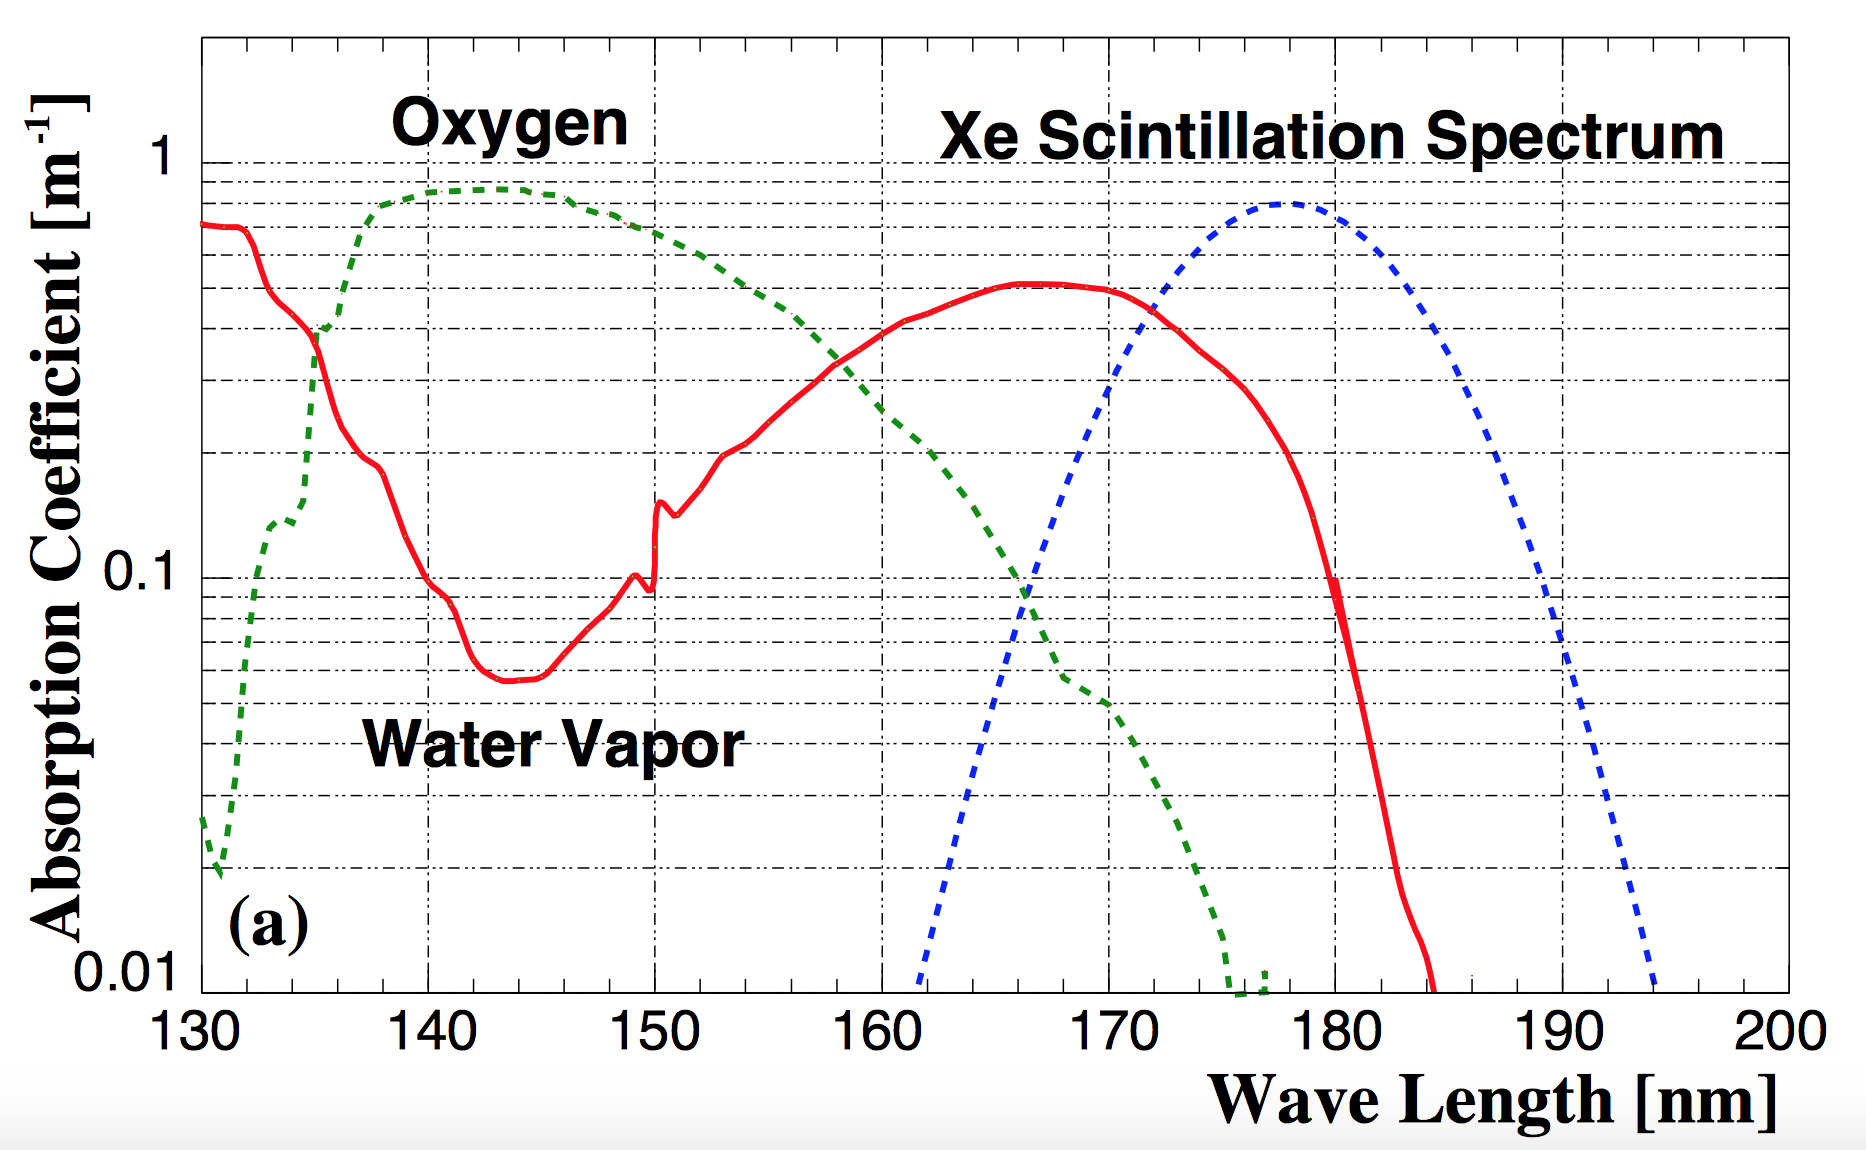
\includegraphics[width=0.8\textwidth]{AbsorptionSpectra}
\caption{Absorption coefficient for photons in 1 ppm \ce{H_2O} vapor (solid red) and \ce{O_2} (dashed green).  The Xe scintillation
spectrum is overlaid for comparison (dashed blue).  \ce{H_2O} impacts Xe scintillation considerably
more than \ce{O_2}.  Image credit: \citeref{Ozone2005}, \ce{H_2O} data from \citeref{Yoshino1996}.}
\label{fig:importance_procedure_effects_photons_absorption_coefficents}
\end{figure}

The relative intensities for different \ce{H_2O}/Xe and \ce{O_2}/Xe concentrations from $0 \mdash 60\ \mathrm{cm}$ are shown in
\figref{fig:importance_procedure_effects_photons_absorption_distance}.  We see that at the level of $\mathcal{O}(100)\ \mathrm{ppb}$ of
oxygen $I / I_0 > 0.8$ at 60 cm.  The effect of water is substantially worse with $I / I_0 < 0.3$, highlighting the necessity of
significant reduction in XENON1T.  Even with a LXe purity that is appreciably better than
\figref{fig:importance_procedure_effects_photons_absorption_distance} $\lambda_{\mathrm{att}} \sim \lambda_{\mathrm{abs}}$ since
the effects of scattering are subdominant with respect to absorption.

\begin{figure}
\centering
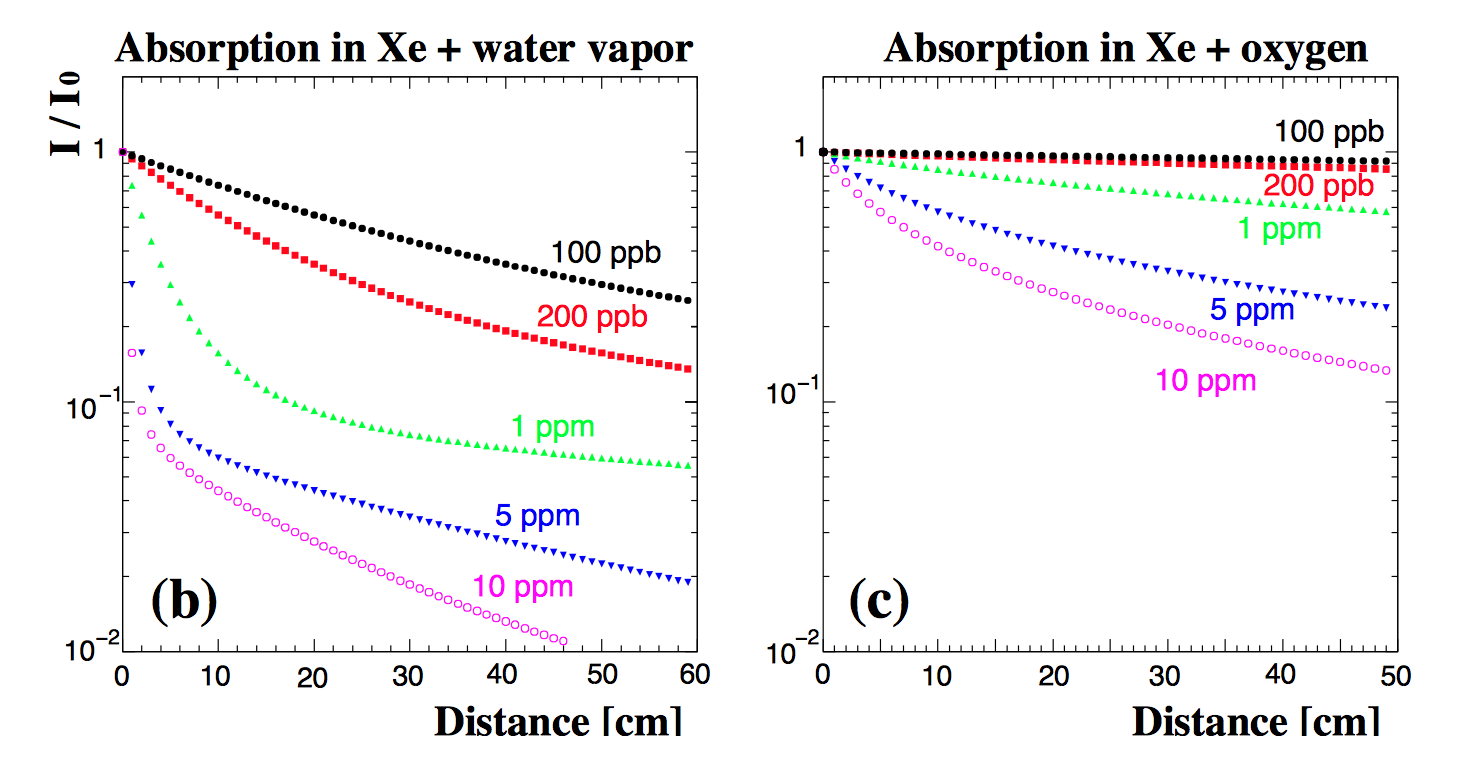
\includegraphics[width=\textwidth]{AbsorptionWithDistance}
\caption{Fraction of initial intensity of xenon scintillation with distance for various concentrations of \htwoo (left) and \otwo
(right).  Image credit: \citeref{Ozone2005}.}
\label{fig:importance_procedure_effects_photons_absorption_distance}
\end{figure}

Photon attenuation ultimately increases our energy threshold as we are less sensitive to lower energies as few photons are
measured.



\subsubsection{Charge Depletion}
\label{subsubsec:importance_procedure_effects_charge}






Page 257 in Aprile book